\chapter{User Guide}

\section{Login screen}

\begin{figure}[H]
  \centering
  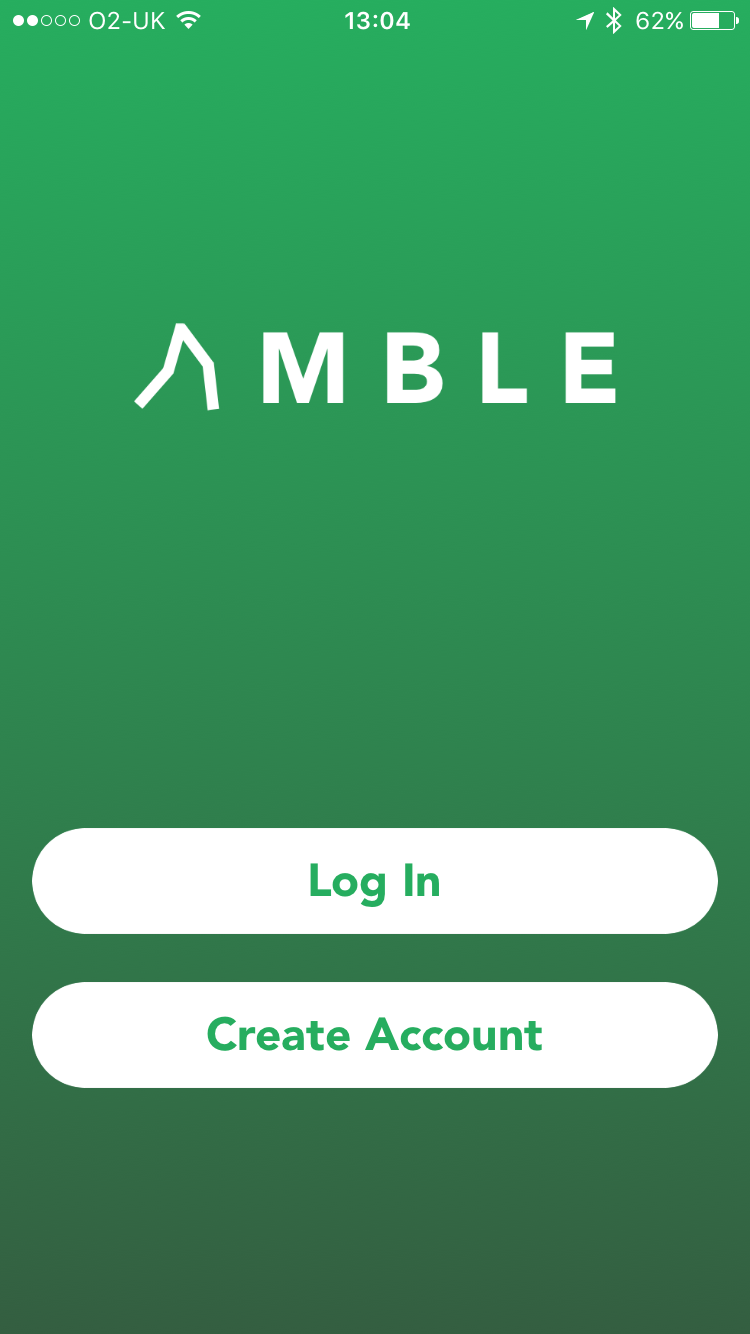
\includegraphics[width=0.375\textwidth]{launch-screen}
  \caption{Initial launch screen shown when launching the app for the first time or when not logged in.}
  \label{fig:launch-screen}
\end{figure}

When you launch the application for the first time, you are greeted with the login initial launch screen shown in Figure \ref{fig:launch-screen}. From here, you can either login to an existing account or create a new one.

Once you choose to login or register, you are taken to the screens displayed in Figure \ref{fig:login-register-screens}. The view on the left prompts you to log in with your username and password, while the view on the right asks you to enter additional details to register an account including your full name and email address.     

\begin{figure}[hbt]
  \centering
  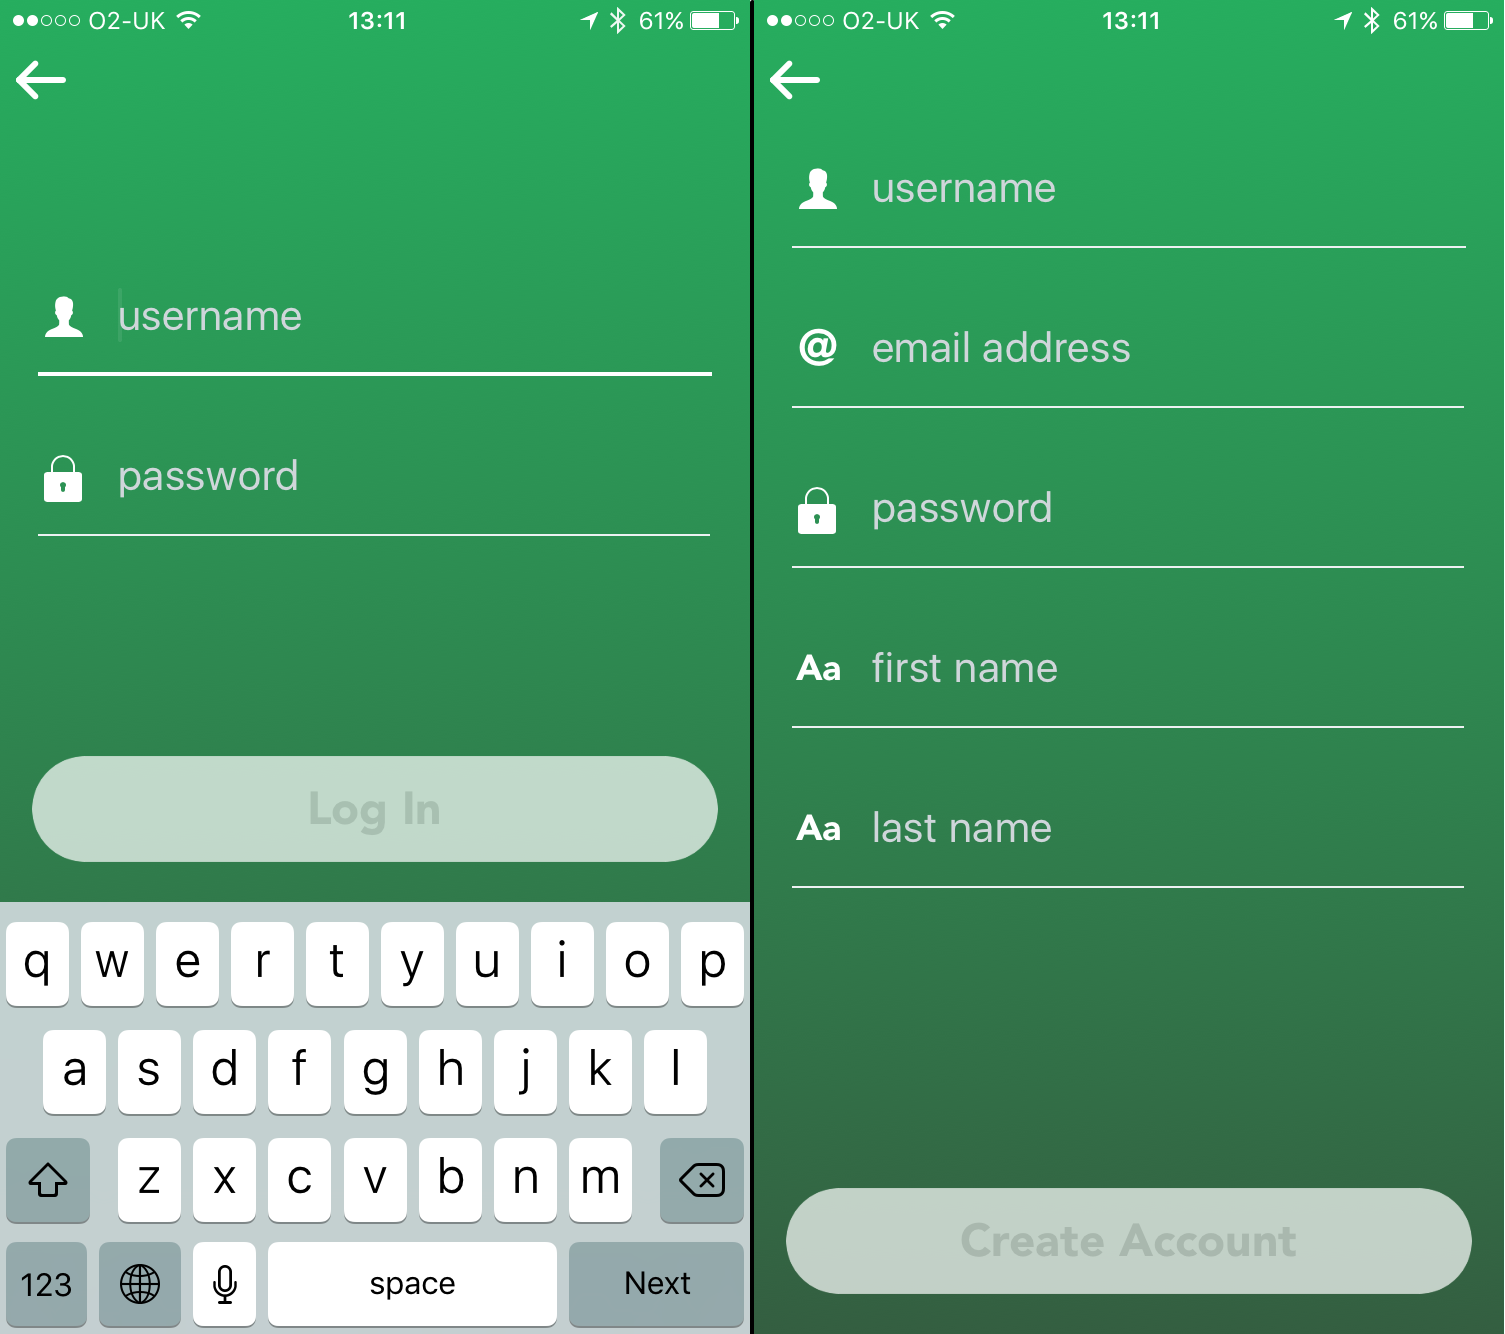
\includegraphics[width=0.7\textwidth]{login-register-screens}
  \caption{Login screen of the app (left) and register screen (right).}
  \label{fig:login-register-screens}
\end{figure}

%Any errors 

\section{Track walks}

Once you have authenticated successfully, you are taken to the main screen of the app shown in Figure \ref{fig:track-walk-screen}, where a map is displayed and walks can be tracked. Here, the app is split into three sections -- the first of which is tracking a walk. As long as you are logged in, you will automatically be taken to this screen when you launch the app.

\begin{figure}[hbt]
  \centering
  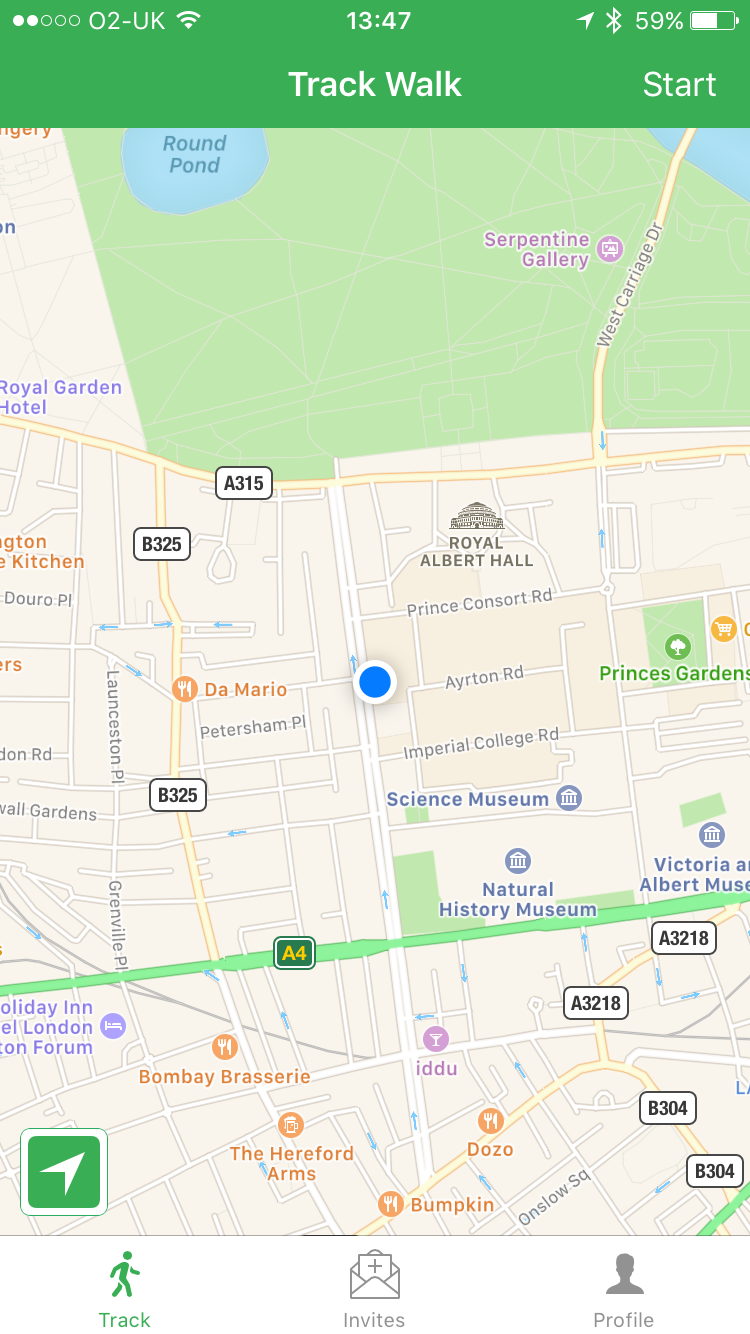
\includegraphics[width=0.375\textwidth]{track-walk-screen}
  \caption{The main screen of the app to track walks, shown after logging in or when launching the app already logged in.}
  \label{fig:track-walk-screen}
\end{figure}


The arrow button in the bottom-left of the screen allows you to toggle between tracking modes -- tapping it once will zoom to your location on the map, and tapping it again will add a compass that will rotate the map as you move your device.

To start tracking a walk, you can tap the \textit{Start} button in the top-right. The app then brings up the statistics view with a timer of the walk duration, the distance travelled during the walk and the number of steps taken. A line is drawn along your route as you begin to walk. Points of interest will also appear around you as you walk along, shown as red pins on the map. The full track walk view can be seen in Figure \ref{fig:track-walk-start}.

\begin{figure}[hbt]
  \centering
  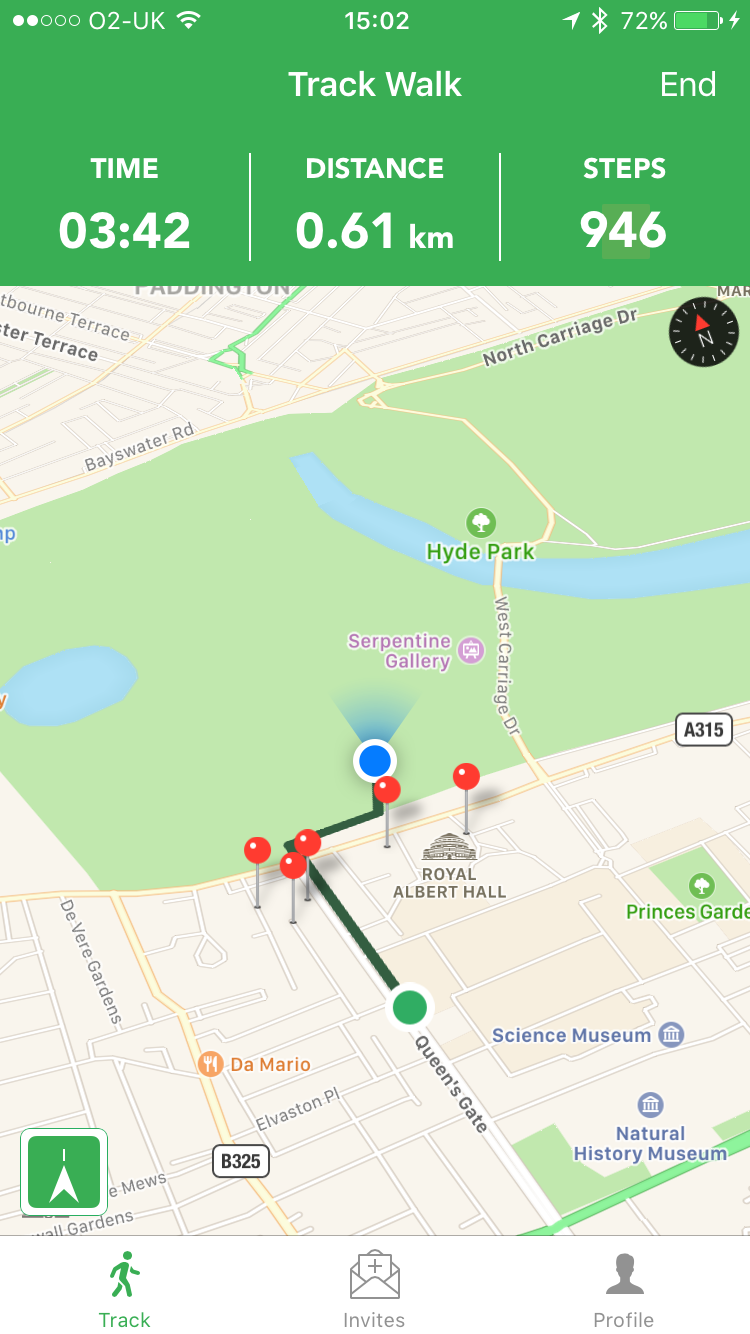
\includegraphics[width=0.375\textwidth]{track-walk-start}
  \caption{The screen displayed while tracking a walk, showing the walk statistics at the top of the screen, a route on the map of where you walk and points of interest displayed around your location as red pins.}
  \label{fig:track-walk-start}
\end{figure}


Tapping on a pin on the map during a walk will result in a popup with a short description and image. To get further information about the point of interest, you can tap the \textit{i} button. This will bring up a screen with more details about the plaque, including its inscription and related person(s). This process is shown in Figure ***.

To save a walk, tap the \textit{End} button in the top-right. This will give you a confirmation message and, once confirmed, will prompt you to enter a name for the walk. Once you enter a name and save the walk, the entire walk will be displayed as shown in Figure \ref{fig:walk-detail-screen}. Here a map is displayed of the entire walk route as well as the walk statistics and achievements, along with the number of points that you gained, listed below.

\begin{figure}[hbt]
  \centering
  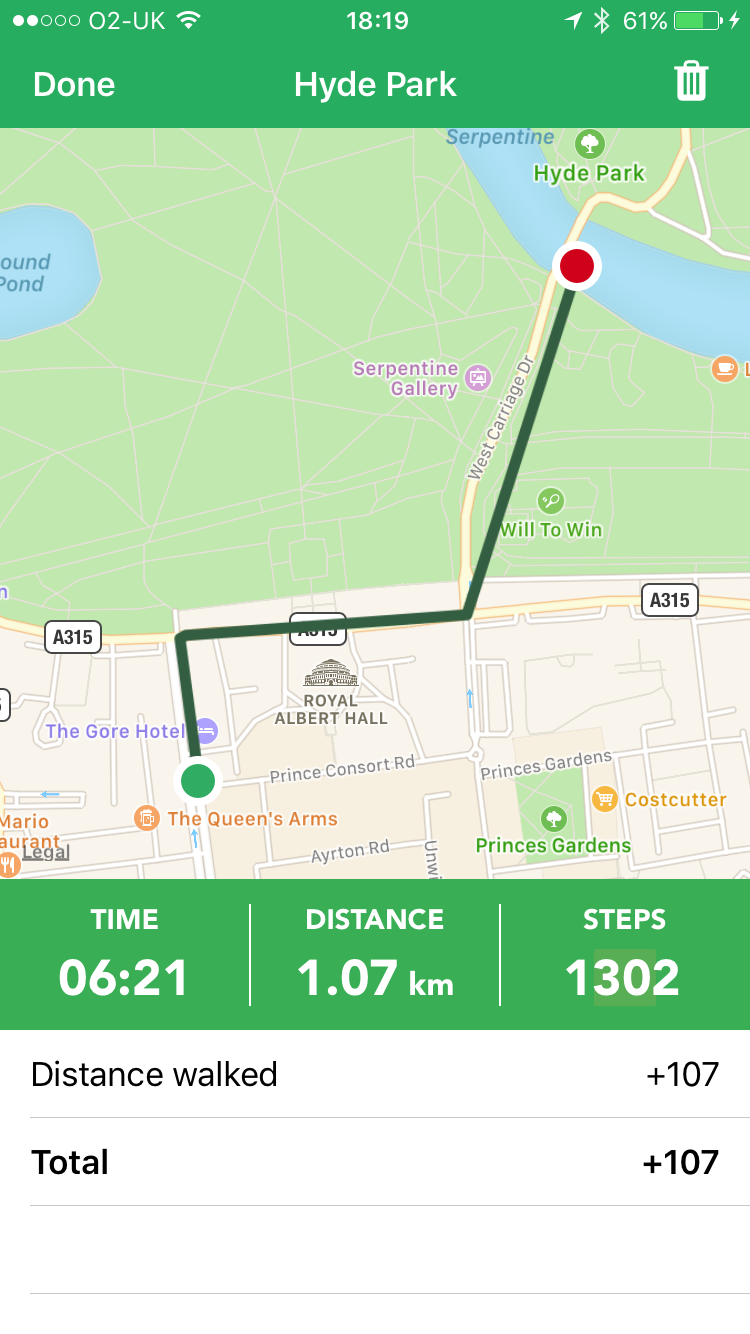
\includegraphics[width=0.375\textwidth]{walk-detail-screen}
  \caption{The walk detail view containing the route of the walk, its statistics and achievements. This view is shown after the walk has been saved (or when selected on your profile).}
  \label{fig:walk-detail-screen}
\end{figure}


\section{Invitations}

The second tab in the application is designed to send and respond to walk invitations. The view initially shows the invites you have sent, with each invite containing a label to show whether the invite is \textit{Pending} or \textit{Accepted}. If a sent invite is marked as accepted, a \textit{Start Walk} button will appear that will switch to the track walk screen and begin tracking a group walk.

By using the toggle at the top of the screen, you can switch to view your received invites. Any pending invitations will be marked with a badge on the tab and a badge on the app's icon. \textit{Accept} and \textit{Decline} buttons are available -- tapping decline will delete the invite and tapping accept will mark it as accepted. Both views can be seen in Figure \ref{fig:invites-screen}.

\begin{figure}[hbt]
  \centering
  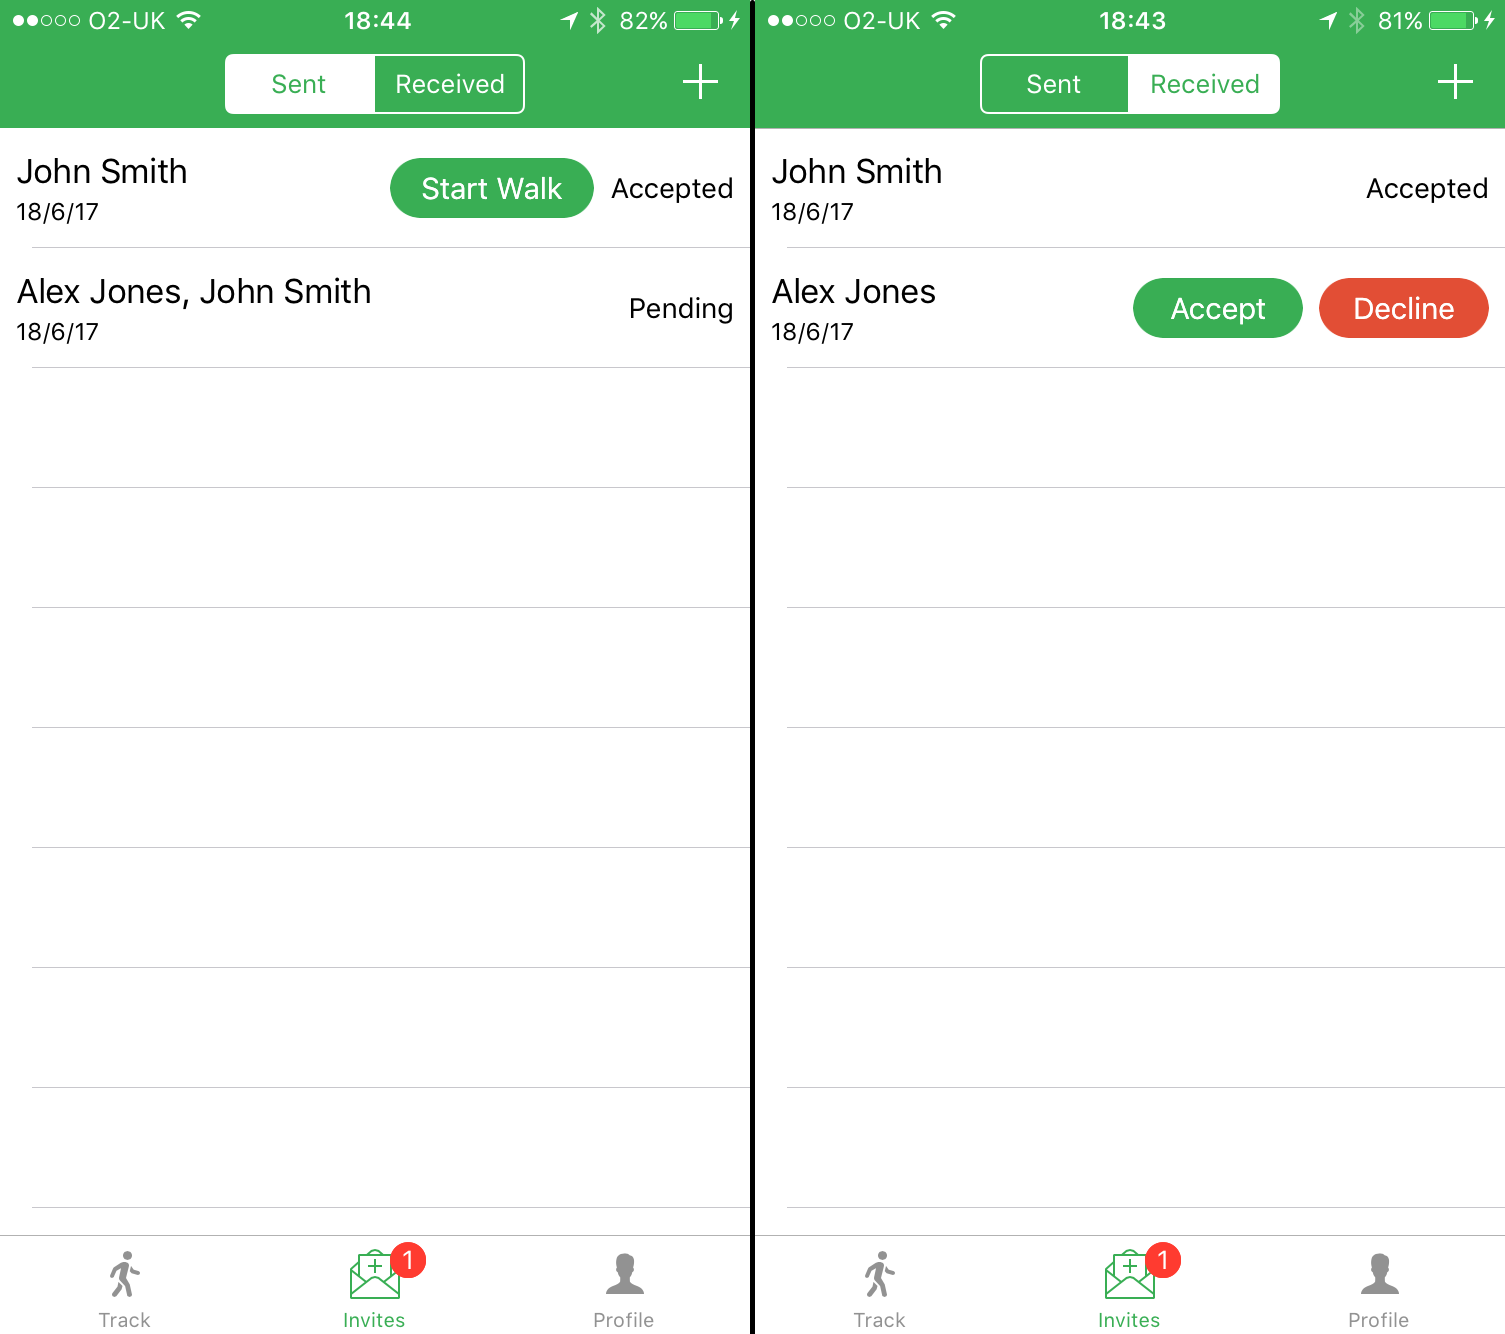
\includegraphics[width=0.7\textwidth]{invites-screen}
  \caption{Invites screen in the app, showing sent invites (left) and received invites (right).}
  \label{fig:invites-screen}
\end{figure}

To invite other users on a walk, tap the \texttt{+} icon in the top-right of the menu bar. This will take you to the screen shown in Figure \ref{fig:invite-user-screen}, with a search bar to search for users by their username, name or email. Once a user is selected from the list of search results, it will appear in the \textit{Selected Users} section. From here you can either perform another search to add more user(s) or tap the \textit{Invite} button in the top-right of the screen to send the invite. You are then returned to the sent invites screen.

\begin{figure}[hbt]
  \centering
  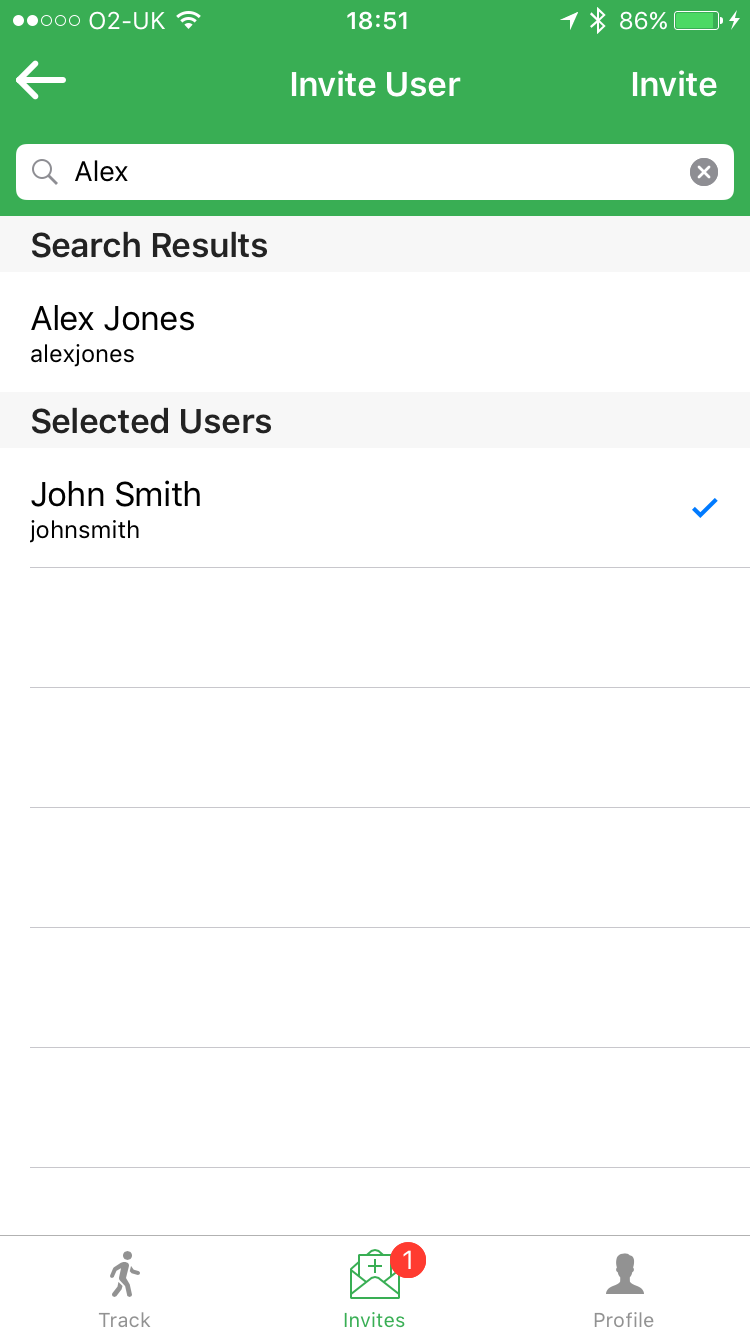
\includegraphics[width=0.375\textwidth]{invite-user-screen}
  \caption{Screen to send an invitation to one or more users.}
  \label{fig:invite-user-screen}
\end{figure}


\section{Profile}

The third tab of the application is your profile view, shown in Figure \ref{fig:profile-screen}. This view displays your user statistics -- specifically your total number of points (or score), the total distance you have walked and your total number of steps taken.

\begin{figure}[hbt]
  \centering
  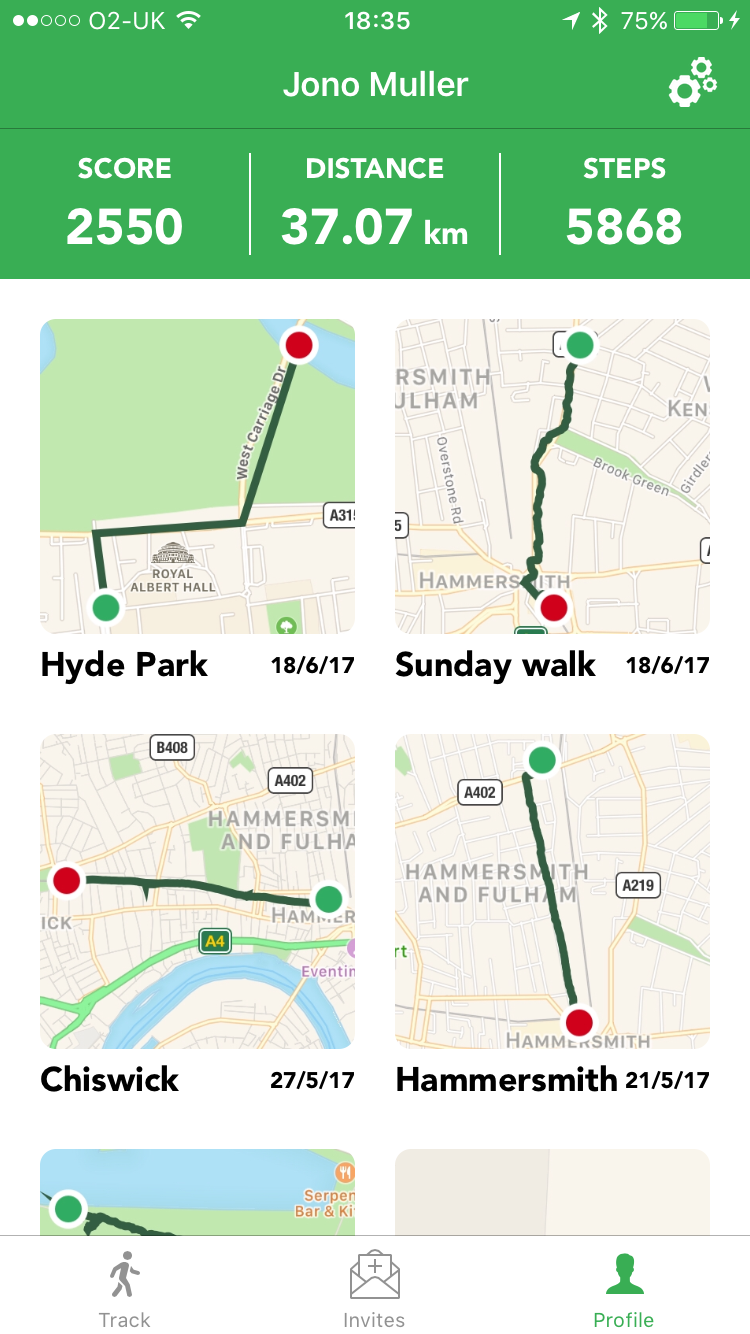
\includegraphics[width=0.375\textwidth]{profile-screen}
  \caption{Profile view in the app, showing your statistics and tracked walks.}
  \label{fig:profile-screen}
\end{figure}


A list of all the walks you have tracked, including group walks, are then shown in a grid formation below. Tapping on a walk will present you with the walk detail view discussed previously (Figure \ref{fig:walk-detail-screen}).

There is also a settings screen accessible via the cog icon on the top-right of the profile view. This gives you the option to change your desired unit of distance and log out, which takes you back to the initial launch screen (Figure \ref{fig:launch-screen}).



